% -*- Mode: LaTeX; Package: CLIM-USER -*-

\chapter {General Designs}
\label {designs}

This chapter discusses more general designs than Chapter~\ref{color} and reveals
that regions are also designs.  This chapter generalizes to those designs that
do not have the same color and opacity at every point in the drawing plane.
These include:

\begin{itemize}
\item composite designs,

\item patterns,

\item stencils,

\item tiled designs,

\item transformed designs,

\item output record designs, and

\item regions
\end{itemize}

Several of the features described in this chapter may not be fully supported in
Release 2 of CLIM.

{\bf Note:} A design is a unification of both a shape and a color and opacity.
As such, a design can serve multiple roles.  For example, the same design can
play the role of an ink that colors the drawing plane, a shape that specifies
where to draw another design, a stencil that controls the compositing of two
designs, the background of a window, or a region that defines clipping.  It is
important not to get confused between \term{type}, which is inherent in an
object, and \term{role}, which is determined by how an object is used in a
particular function call.


\section {The Compositing Protocol}

\concept{Compositing} creates a design whose appearance at each point is a
composite of the appearances of two other designs at that point.  Three
varieties of compositing are provided: \concept{composing over},
\concept{composing in}, and \concept{composing out}.

The methods for \cl{compose-over}, \cl{compose-in}, and \cl{compose-out}
will typically specialize both of the design arguments.

{\sl In Release 2, compositing might only be supported for uniform designs.}


\Defgeneric {compose-over} {design1 design2}

Composes a new design that is equivalent to the \term{design} \arg{design1} on
top of the \term{design} \arg{design2}.  Drawing the resulting design produces
the same visual appearance as drawing \arg{design2} and then drawing
\arg{design1}, but might be faster and might not allow the intermediate state to
be visible on the screen.

If both arguments are regions, \cl{compose-over} is the same as
\cl{region-union}.

\MayCaptureInputs
The result returned by \cl{compose-over} might be freshly constructed or might
be an existing object.


\Defgeneric {compose-in} {ink mask}

Composes a new design by clipping the \term{design} \arg{ink} to the inside of
the \term{design} \arg{mask}.  The first design, \arg{ink}, supplies the color,
while the second design, \arg{mask}, changes the shape of the design by
adjusting the opacity.

More precisely, at each point in the drawing plane the resulting design
specifies a color and an opacity as follows: the color is the same color that
\arg{ink} specifies.  The opacity is the opacity that \arg{ink} specifies,
multiplied by the stencil opacity of \arg{mask}.

The \concept{stencil opacity} of a design at a point is defined as the opacity
that would result from drawing the design onto a fictitious medium whose drawing
plane is initially completely transparent black (opacity and all color
components are zero), and whose foreground and background are both opaque black.
With this definition, the stencil opacity of a member of class \cl{opacity} is
simply its value.

If \arg{mask} is a solid design, the effect of \cl{compose-in} is to clip
\arg{ink} to \arg{mask}.  If \arg{mask} is translucent, the effect is a soft
matte.

If both arguments are regions, \cl{compose-in} is the same as
\cl{region-intersection}.

\MayCaptureInputs
The result returned by \cl{compose-in} might be freshly constructed or might be
an existing object.


\Defgeneric {compose-out} {ink mask}

Composes a new design by clipping the \term{design} \arg{ink} to the outside of
the \term{design} \arg{mask}.  The first design, \arg{ink}, supplies the color,
while the second design, \arg{mask}, changes the shape of the design by
adjusting the opacity.

More precisely, at each point in the drawing plane the resulting design
specifies a color and an opacity as follows: the color is the same color that
\arg{ink} specifies.  The opacity is the opacity that \arg{ink} specifies,
multiplied by 1 minus the stencil opacity of \arg{mask}.

If \arg{mask} is a solid design, the effect of \cl{compose-out} is to clip
\arg{ink} to the complement of \arg{mask}.  If \arg{mask} is translucent, the
effect is a soft matte.

If both arguments are regions, \cl{compose-out} is the same as
\cl{region-difference} of \arg{mask} and \arg{ink}.

\MayCaptureInputs
The result returned by \cl{compose-out} might be freshly constructed or might be
an existing object.


\section {Patterns and Stencils}

\concept{Patterning} creates a bounded rectangular arrangement of designs, like
a checkerboard.  Drawing a pattern draws a different design in each rectangular
cell of the pattern.  To create an infinite pattern, apply
\cl{make-rectangular-tile} to a pattern.

A \concept{stencil} is a special kind of pattern that contains only opacities.

\Defun {make-pattern} {array designs}

Returns a pattern design that has \cl{(array-dimension \arg{array} 0)} cells in
the vertical direction and \cl{(array-dimension \arg{array} 1)} cells in the
horizontal direction.  \arg{array} must be a two-dimensional array of
non-negative integers less than the length of \arg{designs}.  \arg{designs} must
be a sequence of \term{designs}.  The design in cell $(i,j)$ of the resulting
pattern is the $n$th element of \arg{designs}, if $n$ is the value of \cl{(aref
\arg{array} i j)}.  For example, \arg{array} can be a bit-array and
\arg{designs} can be a list of two designs, the design drawn for 0 and the one
drawn for 1.

Each cell of a pattern can be regarded as a hole that allows the design in it to
show through.  Each cell might have a different design in it.  The portion of
the design that shows through a hole is the portion on the part of the drawing
plane where the hole is located.  In other words, incorporating a design into a
pattern does not change its alignment to the drawing plane, and does not apply a
coordinate transformation to the design.  Drawing a pattern collects the pieces
of designs that show through all the holes and draws the pieces where the holes
lie on the drawing plane.  The pattern is completely transparent outside the
area defined by the array.

Each cell of a pattern occupies a 1 by 1 square.  You can use
\cl{transform-region} to scale the pattern to a different cell size and shape,
or to rotate the pattern so that the rectangular cells become diamond-shaped.
Applying a coordinate transformation to a pattern does not affect the designs
that make up the pattern.  It only changes the position, size, and shape of the
cells' holes, allowing different portions of the designs in the cells to show
through.  Consequently, applying \cl{make-rectangular-tile} to a pattern of
nonuniform designs can produce a different appearance in each tile.  The pattern
cells' holes are tiled, but the designs in the cells are not tiled and a
different portion of each of those designs shows through in each tile.

\MayCaptureInputs

\defgeneric {pattern-width} {pattern}
\Defgeneric {pattern-height} {pattern}

These functions return the width and height, respectively, of the \term{pattern}
\arg{pattern}.


\Defun {make-stencil} {array}

Returns a pattern design that has \cl{(array-dimension \arg{array} 0)} cells in
the vertical direction and \cl{(array-dimension \arg{array} 1)} cells in the
horizontal direction.  \arg{array} must be a two-dimensional array of real
numbers between 0 and 1 (inclusive) that represent opacities.  The design in
cell $(i,j)$ of the resulting pattern is the value of \cl{(make-opacity (aref
\arg{array} i j))}.

\MayCaptureInputs


\section {Tiling}

\concept{Tiling} repeats a rectangular portion of a design throughout the
drawing plane.  This is most commonly used with patterns.

\Defun {make-rectangular-tile} {design width height}

Returns a design that, when used as an ink, tiles a rectangular portion of the
\term{design} \arg{design} across the entire drawing plane.  The resulting
design repeats with a period of \arg{width} horizontally and \arg{height}
vertically.  \arg{width} and \arg{height} must both be integers.  The portion of
\arg{design} that appears in each tile is a rectangle whose top-left corner is
at $(0,0)$ and whose bottom-right corner is at $(width,height)$.  The repetition
of \arg{design} is accomplished by applying a coordinate transformation to shift
\arg{design} into position for each tile, and then extracting a \arg{width} by
\arg{height} portion of that design.

Applying a coordinate transformation to a rectangular tile does not change the
portion of the argument \arg{design} that appears in each tile.  However, it can
change the period, phase, and orientation of the repeated pattern of tiles.
This is so that adjacent figures drawn using the same tile have their inks
``line up''.


\section {Regions as Designs}

Any member of the class \cl{region} is a solid, colorless design.  The design is
opaque at points in the region and transparent elsewhere.
Figure~\ref{design-classes} shows how the design and region classes relate to
each other.

\begin{figure}
\centerline{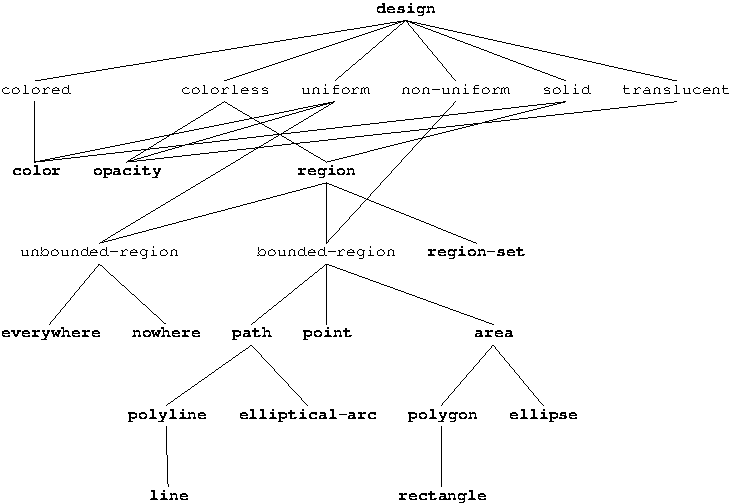
\includegraphics{design-classes}}
\caption{\label{design-classes} The class structure for all designs and regions.
Entries in bold correspond to real CLIM classes.}
\end{figure}

Since bounded designs obey the region protocol, the functions
\cl{transform-region} and \cl{untransform-region} accept any design as their
second argument and apply a coordinate transformation to the design.  The result
is a design that might be freshly constructed or might be an existing object.

Transforming a uniform design simply returns the argument.  Transforming a
composite, flipping, or indirect design applies the transformation to the
component design(s).  Transforming a pattern, tile, or output record design is
described in the sections on those designs.


\section {Arbitrary Designs}

\Defgeneric {draw-design} {medium design \key \DrawingOptions \LineJointCapOptions\ \TextOptions}

Draws the \term{design} \arg{design} onto the \term{medium} \arg{medium}.  This is
defined to work for all types of regions and designs, although in practice some
implementations may be more restrictive.  \arg{ink}, \arg{transformation}, and
\arg{clipping-region} are used to modify the medium.  The other drawing
arguments control the drawing of the design, depending on what sort of design is
being drawn.  For instance, if \arg{design} is a path, then line style options
may be supplied.

If \arg{design} is an area, \cl{draw-design} paints the specified region of the
drawing plane with medium's current ink.  If \arg{design} is a
path, \cl{draw-design} strokes the path with medium's current ink under control
of the line-style.  If \arg{design} is a point, \cl{draw-design} is the same as
\cl{draw-point}.

If \arg{design} is a color or an opacity, \cl{draw-design} paints the entire
drawing plane (subject to the clipping region of the medium).

If \arg{design} is \cl{+nowhere+}, \cl{draw-design} has no effect.

If \arg{design} is a non-uniform design (see Chapter~\ref{designs}),
\cl{draw-design} paints the design, positioned at coordinates $(0,0)$.

CLIM implementations are required to support \cl{draw-design} for the following
cases:

\begin{itemize}
\item Designs created by the geometric object constructors, such as
\cl{make-line} and \cl{make-ellipse}, in conjunction with drawing arguments that
supply the drawing ink.

\item Designs created by calling \cl{compose-in} on a color and an object
created by a geometric object constructor.

\item Designs created by calling \cl{compose-over} on any of the cases above.

\item Designs returned by \cl{make-design-from-output-record}.
\end{itemize}


\Defun {draw-pattern*} {medium pattern x y \key clipping-region transformation}

Draws the pattern \arg{pattern} on the \term{medium} \arg{medium} at the
position $(x,y)$. \arg{pattern} is any design created by \cl{make-pattern}.
\arg{clipping-region} and \arg{transformation} are as for
\cl{with-drawing-options} or any of the drawing functions.

Note that \arg{transformation} only affects the position at which the pattern is
drawn, not the pattern itself.  If a programmer wishes to affect the pattern, he
should explicity call \cl{transform-region} on the pattern.

Drawing a bitmap consists of drawing an appropriately aligned and scaled pattern
constructed from the bitmap's bits.  A 1 in the bitmap corresponds to
\cl{+foreground-ink+}, while a 0 corresponds to \cl{+background-ink+} if an
opaque drawing operation is desired, or to \cl{+nowhere+} if a transparent
drawing operation is desired.

Drawing a (colored) raster image consists of drawing an appropriately aligned
and scaled pattern constructed from the raster array and raster color map.

\cl{draw-pattern*} could be implemented as follows, assuming that the functions
\cl{pattern-width} and \cl{pattern-height} return the width and height of the
pattern.

\begin{verbatim}
(defun draw-pattern* (medium pattern x y &key clipping-region transformation)
  (check-type pattern pattern)
  (let ((width (pattern-width pattern))
        (height (pattern-height pattern)))
    (if (or clipping-region transformation)
        (with-drawing-options (medium :clipping-region clipping-region
                                      :transformation transformation)
          (draw-rectangle* medium x y (+ x width) (+ y height)
                           :filled t :ink pattern))
        (draw-rectangle* medium x y (+ x width) (+ y height)
                         :filled t :ink pattern))))
\end{verbatim}


\section {Examples of More Complex Drawing Effects}

\paragraph {Painting a gray or colored wash over a display.}

Specify a translucent design as the ink, such as \cl{:ink (compose-in +black+
(make-opacity 0.25))}, \cl{:ink (compose-in +red+ (make-opacity 0.1))}, or
\cl{:ink (compose-in +foreground-ink+ (make-opacity 0.75))}.  The last example
can be abbreviated as \cl{:ink (make-opacity 0.75)}.  On a non-color,
non-grayscale display this will usually turn into a stipple.

\paragraph {Drawing a faded but opaque version of the foreground color.}

Specify \cl{:ink (compose-over (compose-in +foreground-ink+ (make-opacity 0.25))
+background-ink+)} to draw at 25\% of the normal contrast.  On a non-color,
non-grayscale display this will probably turn into a stipple.

\paragraph {Drawing a tiled pattern.}

Specify \cl{:ink (make-rectangular-tile (make-pattern \arg{array} \arg{colors}))}.

\paragraph {Drawing a ``bitmap''.}

Use \cl{(draw-design \arg{medium} (make-pattern \arg{bit-array} (list
+background-ink+ +foreground-ink+)) :transformation
(make-translation-transformation \arg{x} \arg{y}))}.


\section {Design Protocol}

\issue {SWM} {The generic functions underlying the functions described in this
and the preceding chapter will be documented later.  This will allow for
programmer-defined design classes.  This also needs to describe how to decode
designs into inks.}
